\documentclass[a4paper,12pt,twocolumn]{article}
\usepackage{geometry}
\geometry{margin=0.5in}
\usepackage[utf8]{inputenc}
\usepackage[most]{tcolorbox}
\usepackage{chemmacros}
\usepackage{graphicx}
\usepackage[version=4]{mhchem}
\usepackage{nopageno}
\usepackage{tikz}

\newtcolorbox{Box1}[2][]{
                lower separated=false,
                colback=white!80!gray,
colframe=white, fonttitle=\bfseries,
colbacktitle=white!50!gray,
coltitle=black,
enhanced,
attach boxed title to top left={xshift=0.5cm,yshift=-2mm},
title=#2,#1}


\newtcolorbox{Box2}[2][]{
                lower separated=false,
                colback=white,
colframe=black,fonttitle=\bfseries,
colbacktitle=black,
coltitle=white,
enhanced,
attach boxed title to top left={yshift=-0.1in,xshift=0.15in},
                 boxed title style={boxrule=0pt,colframe=white,},
title=#2,#1}

\newtcolorbox{Box3}[2][]{
                lower separated=false,
                colback=white!80!gray,
colframe=white!20!black,fonttitle=\bfseries,
colbacktitle=white!30!gray,
coltitle=black,
enhanced,
attach boxed title to top left={xshift=0.5cm,
        yshift=-2mm},
title=#2,#1}

\newtcolorbox{Box4}[2][]{arc=0mm,
                lower separated=false,
                colback=white!80!gray,
colframe=white!20!black,fonttitle=\bfseries,
colbacktitle=white!30!gray,
coltitle=black,
enhanced,
attach boxed title to top left={xshift=0.5cm,
        yshift=-2mm},
title=#2,#1}

\newcommand{\oxi}[2]{%
    \stackrel{#1}{\mathrm{#2}}
}%
\DeclareUnicodeCharacter{2212}{-}

\begin{document}

\begin{center}
    \huge{Chemical Equilibrium} 
\end{center}

\section{Equilibrium}
\begin{itemize}
    \item Equilibrium is a state in which there are no observable changes as time goes by.
    \item When a chemical reaction has reached the equilibrium state, the concentrations of reactants and products remain constant over time, and there are no visible changes in the system. 
    \item However, there is much activity at the molecular level because reactant molecules continue to form product molecules while product molecules react to yield reactant molecules.
\end{itemize}

\section{Physical Equilibrium}
\begin{itemize}
    \item Equilibrium between two phases of the same substance is called physical equilibrium because the changes that occur are physical processes. 
    \item The vaporization of water in a closed container at a given temperature is an example of physical equilibrium. In this instance, the number of H2O molecules leaving and the number returning to the liquid phase are equal:
          \begin{center}
            $\ce{H2O (l) <=> H2O (g)}$
          \end{center}
    \item The study of physical equilibrium yields useful  information, such as the equilibrium vapor pressure.
\end{itemize}

\section{Chemical Equilibrium}
\begin{itemize}
    \item Few chemical reactions proceed in only one direction. Most are reversible, at least to some extent. At the start of a reversible process, the reaction proceeds toward the formation of products. As soon as some product molecules are formed, the reverse process begins to take place and reactant molecules are formed from product molecules.
    \item \textbf{Chemical equilibrium} is achieved when the rates of the forward and reverse reactions are equal and the concentrations of the reactants and products remain constant.
    \item Chemical equilibrium is a \textbf{dynamic process}.
\end{itemize}

\section{Dynamic Equilibrium}
\begin{itemize}
    \item A dynamic equilibrium exists once a reversible reaction occurs. 
    \item Substances undergo transition between the reactants and products at equal rates, meaning there is no net change. Reactants and products are formed at such a rate that the concentration of neither changes. 
    \item It is a particular example of a system in a steady state.
\end{itemize}

\section{Chemical Equilibrium processes}
\begin{itemize}
    \item Reversible reaction involving nitrogen dioxide ($\ce{NO2}$) and dinitrogen tetroxide ($\ce{N2O4}$). The progress of the reaction
          \begin{center}
            $\ce{N2O4 (g) <=> 2NO2 (g)}$
          \end{center}
          can be monitored easily because $\ce{N2O4}$ is a colorless gas, whereas $\ce{NO2}$ has a dark brown color.\\
\end{itemize}
\begin{figure}[h]
    \centering
    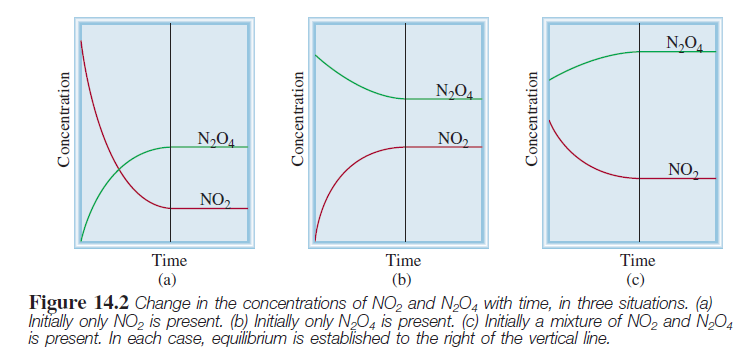
\includegraphics[width=.5\textwidth]{Screenshot 2023-03-22 021052.png}
\end{figure}

\begin{table}[h!]
    \centering
    \small 
    \begin{tabular}{|p{1.1cm}|p{1.1cm}|p{1.1cm}|p{1.1cm}|p{1cm}|p{2cm}|}
        \hline \multicolumn{2}{|p{2.2cm}|}{$\begin{array}{c}\text {Initial} \\
        \text {Concentrations} \\
        (M)\end{array}$} & \multicolumn{2}{|p{2.2cm}|}{$\begin{array}{c}\text {Equilibrium} \\
        \text {Concentrations} \\
        (M)\end{array}$} & \multicolumn{2}{|c|}{$\begin{array}{c}\text {Ratio of} \\
        \text {Concentrations} \\
        \text {at Equilibrium}\end{array}$} \\
        \hline$\left[\mathrm{NO}_2\right]$ & {$\left[\mathrm{N}_2 \mathrm{O}_4\right]$} & {$\left[\mathrm{NO}_2\right]$} & {$\left[\mathrm{N}_2 \mathrm{O}_4\right]$} & $\dfrac{\left[\mathrm{NO}_2\right]}{\left[\mathrm{N}_2 \mathrm{O}_4\right]}$ & $\dfrac{\left[\mathrm{NO}_2\right]^2}{\left[\mathrm{N}_2 \mathrm{O}_4\right]}$ \\
        \hline 0.000                       & 0.670                                      & 0.0547                         & 0.643                                      & 0.0851                                                                       & $4.65 \times 10^{-3}$                                                          \\
        \hline 0.0500                      & 0.446                                      & 0.0457                         & 0.448                                      & 0.102                                                                        & $4.66 \times 10^{-3}$                                                          \\
        \hline 0.0300                      & 0.500                                      & 0.0475                         & 0.491                                      & 0.0967                                                                       & $4.60 \times 10^{-3}$                                                          \\
        \hline 0.0400                      & 0.600                                      & 0.0523                         & 0.594                                      & 0.0880                                                                       & $4.60 \times 10^{-3}$                                                          \\
        \hline 0.200                       & 0.000                                      & 0.0204                         & 0.0898                                     & 0.227                                                                        & $4.63 \times 10^{-3}$                                                          \\
        \hline
    \end{tabular}
    \caption{$\mathrm{The \quad \ce{NO2 - N2O4} \quad System \quad at \quad 25^oC}$}
\end{table}

\section{Equilibrium Constant}
\begin{itemize}
    \item 
          \begin{center} $\ce{aA + bB <=> cC + dD}$ \end{center}
          For the reaction at a particular temperature
          \begin{center}
            $K = \dfrac{[C]^c[D]^d}{[A]^a[B]^b}$
          \end{center}
    \item It is the mathematical expression of their \textbf{law of mass action}, which holds that for a reversible reaction at equilibrium and a constant temperature, a certain ratio of reactant and product concentrations has a constant value, K (the equilibrium constant).
    \item Note that although the concentrations may vary, as long as a given reaction is at equilibrium and the temperature does not change, according to the law of mass action, the value of K remains constant.
\end{itemize}

\section{Law of Mass Action}
\begin{itemize}
    \item The law of mass action is the proposition that the rate of the chemical reaction is directly proportional to the product of the activities or concentrations of the reactants. 
    \item It explains and predicts behaviors of solutions in dynamic equilibrium. 
    \item Specifically, it implies that for a chemical reaction mixture that is in equilibrium, the ratio between the concentration of reactants and products is constant.
    \item Two aspects are involved in the formulation of the law:
          \begin{enumerate}
            \item the equilibrium aspect, concerning the composition of a reaction mixture at equilibrium.
            \item the kinetic aspect, concerning the rate equations for elementary reactions.
          \end{enumerate}
    \item Chemical equilibrium is a dynamic process in which rates of reaction for the forward and backward reactions must be equal at chemical equilibrium.
\end{itemize}

\section{Equilibrium Constant - A Quotient}
\begin{itemize}
    \item The equilibrium constant is defined by a \\ \textbf{quotient}.
    \item The magnitude of the equilibrium constant tells us whether an equilibrium reaction favors the products or reactants. 
    \item If K is much greater than 1 (that is, $K >>1$), the equilibrium will lie to the right and favors the products. 
    \item Conversely, if the equilibrium constant is much smaller than 1 (that is, $K << 1$), the equilibrium will lie to the left and favor the reactants.\\
          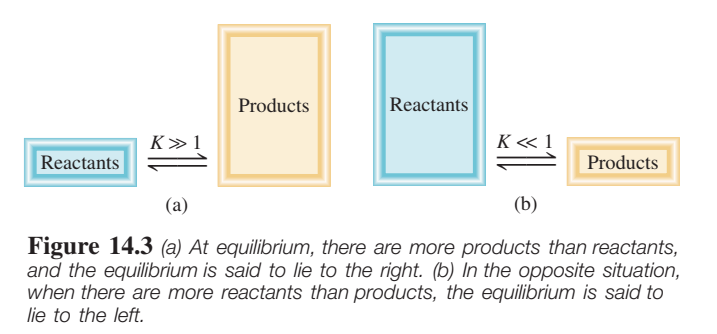
\includegraphics[width=.5\textwidth]{Screenshot 2023-03-23 005954.png}
    \item Any number greater than 10 is considered to be much greater than 1, and any number less than 0.1 is much less than 1.
\end{itemize}

\section{Writing Equilibrium Constant Expressions}
\begin{itemize}
    \item \textbf{Homogenous Equilibria:} Homogeneous equilibrium applies to reactions in which all reacting species are in the same phase.
          \begin{center}
            $\ce{N2O4 (g) <=> 2NO2 (g)}$
          \end{center}
    \item $\mathrm{K_C}$ indicates that the concentrations of the reacting species are expressed in molarity or moles per liter.
          \begin{center}
            $\mathrm{K_C} = \dfrac{[\ce{NO2}]^2}{[\ce{N2O4}]}$
          \end{center}
    \item $\mathrm{K_P}$ tells us that equilibrium concentrations are expressed in terms of pressure.
          \begin{center}
            $\mathrm{K_P} = \dfrac{\mathrm{P^2_{NO_2}}}{\mathrm{P_{N_2O_4}}}$
          \end{center}
\end{itemize}

\section{Relationship Between $K_C$ and $K_P$}
\begin{center}
    $\ce{aA (g) <=> bB (g)}$
\end{center}
We can write the relationship between $K_P$ and $K_C$ as
\begin{center}
    $\mathrm{K_{P}=K_{\mathrm{c}}(RT)^{\Delta n}}$
\end{center}
where,
\\
$\begin{aligned}
    \quad \quad \Delta n & = b-a                                  \\
    \quad \quad          & = \textbf{moles of gaseous products} - \\ 
    \quad \quad          & \textbf{moles of gaseous reactants}    
\end{aligned}$
\\
The gas constant R is given by $0.0821 L.atm/K.mol$, Because pressures are usually expressed in atm.
\section{$K_P = K_C ?$}
In general $\mathrm{K_P \neq K_C ?}$, except in the special case in which $\Delta n  = 0$ as in the equilibrium mixture of molecular hydrogen, molecular bromine and hydrogen bromide:\\ 
\begin{center}
    $\ce{H2 (g) + Br2 (g) <=> 2HBr (g)}$
\end{center}
In this case, we can write, \\
 
$\begin{aligned}
    \quad \quad \quad \quad K_{P} & =K_{c}(0.0821 T)^{0} \\
    \quad \quad \quad \quad       & =K_{c}               
\end{aligned}$
\section{Equilibrium Constant and Units}
\begin{itemize}
    \item It is general practice not to include units for the equilibrium constant. 
    \item In thermodynamics, the equilibrium constant is defined in terms of activities rather than concentrations. 
    \item For an \textbf{ideal system}, the activity of a substance is the ratio of its concentration (or partial pressure) to a standard value, which is 1 M (or 1 atm). This procedure eliminates all units but does not alter the numerical parts of the concentration or pressure. Consequently, K has no units.
    \item For \textbf{nonideal systems}, the activities are not exactly numerically equal to concentrations. In some cases, the differences can be appreciable.
\end{itemize}

\section{Heterogeneous Equilibria}
\begin{itemize}
    \item A heterogeneous equilibrium results from a reversible reaction involving reactants and products that are in different phases.
          \begin{center}
            $\ce{CaCO3 (s) <=> CaO (s) + CO2 (g)}$
          \end{center}
    \item The situation becomes simpler if we replace concentrations with activities. In thermodynamics, \textbf{the activity of a pure solid is 1}. Thus, the concentration terms for $\ce{CaCO3}$ and $\ce{CaO}$ are both unity, and from the preceding equilibrium equation, we can immediately write $\mathrm{K_c} = [\ce{CO2}]$. \\
          \begin{center}
            $\begin{array}{l}
                \mathrm{K^{\prime}_C} = \dfrac{[\ce{CaO}][\ce{CO2}]}{[\ce{CaCO3}]}              \\
                \Rightarrow \mathrm{K^{\prime}_C} \dfrac{[\ce{CaCO3}]}{[\ce{CaO}]} = [\ce{CO2}] \\
                \Rightarrow \mathrm{K_C} = [\ce{CO2}]                                           
            \end{array}$
          \end{center}
          also,
          \begin{center}
            $\mathrm{K_P = P_{CO_2}}$
          \end{center}
    \item Similarly, \textbf{the activity of a pure liquid is also 1}. Thus, if a reactant or a product is a liquid, we can omit it in the equilibrium constant expression.
\end{itemize}

\section{What Does Equilibrium Constant Tell Us?}
\begin{itemize}
    \item Once we know the value of the equilibrium constant, we can calculate unknown equilibrium concentrations—remembering that the equilibrium constant has a constant value only if the temperature does not change. 
    \item In general, the equilibrium constant helps us to predict the direction in which a reaction mixture will proceed to achieve equilibrium and to calculate the concentrations of reactants and products once equilibrium has been reached. 
\end{itemize}

\section{Predecting the Direction of a Reaction}
\begin{itemize}
    \item For reactions that have not reached equilibrium, we obtain the reaction quotient (\(Q_C)\)), instead of the equilibrium constant by substituting the initial concentrations into the equilibrium constant expression.
    \item To determine the direction in which the net reaction will proceed to achieve equilibrium, we compare the values of \(Q_C\) and \(K_C\).
          \begin{table}[h]
            \centering
            \def\arraystretch{1.5}
            \begin{tabular}{|l|p{2.3in}|}
                \hline
                Possibilites         & Outcome                                                               \\ \hline
                $\mathrm{Q_C < K_C}$ & The ratio of initial concentrations of products to reactants is too   
                small. To reach equilibrium, reactants must be converted to products.
                The system proceeds from left to right (consuming reactants,
                forming products) to reach equilibrium. \\ \hline
                $\mathrm{Q_C = K_C}$ & The initial concentrations are equilibrium concentrations. The system 
                is at equilibrium. \\ \hline
                $\mathrm{Q_C > K_C}$ & The ratio of initial concentrations of products to reactants is too   
                large. To reach equilibrium, products must be converted to reactants.
                The system proceeds from right to left (consuming products, forming
                reactants) to reach equilibrium. \\ \hline
            \end{tabular}
            \caption{$\mathrm{Relation\quad Between \quad Q_C \quad and \quad K_C}$}
          \end{table}
\end{itemize}

\section{Factors That Affect Chemical Equilibrium}
\begin{itemize}
    \item Chemical equilibrium represents a balance between forward and reverse reactions. In most cases, this balance is quite delicate. 
    \item Changes in experimental conditions may disturb the balance and shift the equilibrium position so that more or less of the desired product is formed. 
    \item Variables that can be controlled experimentally are concentration, pressure, volume, and temperature.
    \item Examination of the effect of a catalyst on equilibrium is also important.
          
\end{itemize}

\section{Le Châtelier’s Principle}
\begin{itemize}
    \item There is a general rule that helps us to predict the direction in which an equilibrium reaction will move when a change in concentration, pressure, volume, or temperature occurs. 
    \item \textbf{Le Châtelier’s principle} states that \textbf{if an external stress is applied to a system at equilibrium, the system adjusts in such a way that the stress is partially offset as the system reaches a new equilibrium position.}
    \item The word “stress” here means a change in concentration, pressure, volume, or temperature that removes the system from the equilibrium state. 
          
\end{itemize}

\section{Change in Concentration}
Iron(III) thiocyanate $\left[\mathrm{Fe}(\mathrm{SCN})_3\right]$ dissolves readily in water to give a red solution. The red color is due to the presence of hydrated $\mathrm{FeSCN}^{2+}$ ion. The equilibrium between undissociated $\mathrm{FeSCN}^{2+}$ and the $\mathrm{Fe}^{3+}$ and $\mathrm{SCN}^{-}$ions is given by
$$
\begin{array}{ccc}
    \mathrm{FeSCN}^{2+}(a q) \rightleftharpoons & \mathrm{Fe}^{3+}(a q) & + \quad \mathrm{SCN}^{-}(a q) \\
    \text { red }                               & \text { pale yellow}  & \text{ colorless }            
\end{array}
$$
\begin{center}
    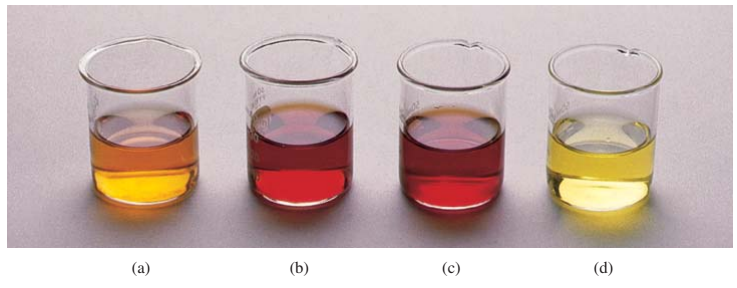
\includegraphics[width=.5\textwidth]{Screenshot 2023-03-23 001124.png}
\end{center}

Effect of concentration change on the position of equilibrium. (a) $A n$ aqueous $\mathrm{Fe}(\mathrm{SCN})_3$ solution. The color of the solution is due to both the red $\mathrm{FeSCN}^{2+}$ and the yellow $\mathrm{Fe}^{3+}$ ions. (b) After the addition of some NaSCN to the solution in (a), the equilibrium shifts to the left. (c) After the addition of some $\mathrm{Fe}\left(\mathrm{NO}_3\right)_3$ to the solution in (a), the equilibrium shifts to the left.
(d) After the addition of some $\mathrm{H}_2 \mathrm{C}_2 \mathrm{O}_4$ to the solution in (a), the equilibrium shifts to the right.
The yellow color is due to the $\mathrm{Fe}\left(\mathrm{C}_2 \mathrm{O}_4\right)_3^{3-}$ ions.
\begin{center}
    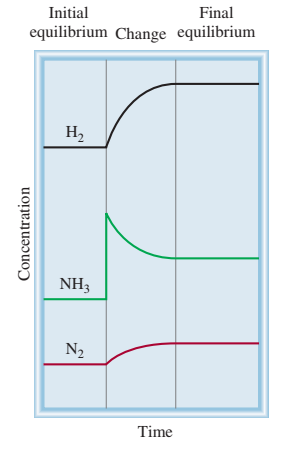
\includegraphics[width=2.5in, height=4in]{Screenshot 2023-03-23 001500.png}
\end{center}
Changes in 
concentration of $\ce{H2}$, $\ce{N2}$, and $\ce{NH3}$ after the addition of $\ce{NH3}$ to the equilibrium mixture. When the new equilibrium is established, all the concentrations are changed but $\mathrm{K_C}$ remains the same because temperature remains constant.
\section{Changes in Volume and Pressure}
\begin{itemize}
    \item Changes in pressure ordinarily do not affect the concentrations of reacting species in 
          condensed phases (say, in an aqueous solution) because liquids and solids are virtually 
          incompressible. On the other hand, concentrations of gases are greatly affected by 
          changes in pressure.
          \begin{center}
            $\mathrm{P V  =n R T}$ \\
          \end{center}
          \begin{center}
            $\mathrm{P  =\left(\dfrac{n}{V}\right) R T}$
          \end{center}
          Note that P and V are related to each other inversely: The greater the pressure, the 
          smaller the volume, and vice versa. Note, too, that the term (n/V) is the concentration 
          of the gas in mol/L, and it varies directly with pressure.
          \begin{center}
            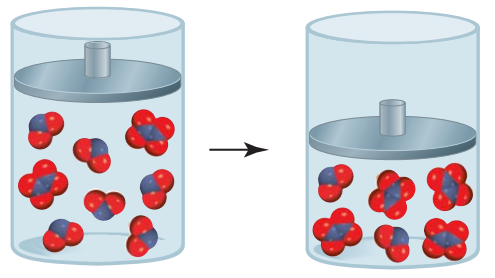
\includegraphics[width=.3\textwidth]{Screenshot 2023-03-22 235304.png}
          \end{center}
          Suppose that the equilibrium system
          $$
          \mathrm{N}_2 \mathrm{O}_4(g) \rightleftharpoons 2 \mathrm{NO}_2(g)
          $$
          is in a cylinder fitted with a movable piston. What happens if we increase the pressure on the gases by pushing down on the piston at constant temperature? Because the volume decreases, the concentration $(n / V)$ of both $\mathrm{NO}_2$ and $\mathrm{N}_2 \mathrm{O}_4$ increases. Note that the concentration of $\mathrm{NO}_2$ is squared in the equilibrium constant expression, so the increase in pressure increases the numerator more than the denominator. The system is no longer at equilibrium and we write
          $$
          Q_{\mathrm{c}}=\frac{\left[\mathrm{NO}_2\right]_0^2}{\left[\mathrm{~N}_2 \mathrm{O}_4\right]_0}
          $$
          Thus, $Q_{\mathrm{c}}>K_{\mathrm{c}}$ and the net reaction will shift to the left until $Q_{\mathrm{c}}=K_{\mathrm{c}}$. Conversely, a decrease in pressure (increase in volume) would result in $Q_{\mathrm{c}}<K_{\mathrm{c}}$, and the net reaction would shift to the right until $Q_{\mathrm{c}}=K_{\mathrm{c}}$. (This conclusion is also predicted by Le Châtelier's principle.)
          
    \item In general, an increase in pressure (decrease in volume) favors the net reaction that decreases the total number of moles of gases (the reverse reaction, in this case), and a decrease in pressure (increase in volume) favors the net reaction that increases the total number of moles of gases (here, the forward reaction). 
    \item For reactions in which there is no change in the number of moles of gases, a pressure (or volume) change has no effect on the position of equilibrium.
    \item It is possible to change the pressure of a system without changing its volume. 
    \item Suppose the $\ce{NO2} – \ce{N2O4}$ system is contained in a stainless-steel vessel whose volume is constant. We can increase the total pressure in the vessel by adding an inert gas (helium, for example) to the equilibrium system. 
    \item Adding helium to the equilibrium mixture at constant volume increases the total gas pressure and decreases the mole fractions of both $\ce{NO2}$ and $\ce{N2O4}$; but the partial pressure of each gas, given by the product of its mole fraction and total pressure does not change. 
    \item Thus, the presence of an inert gas in such a case does not affect the equilibrium.
\end{itemize}

\section{Changes in Temperature}
\begin{itemize}
    \item A change in concentration, pressure, or volume may alter the equilibrium position, that is, the relative amounts of reactants and products, but it does not change the value of the equilibrium constant. 
    \item Only a change in temperature can alter the equilibrium constant.
\end{itemize}
\begin{center}
    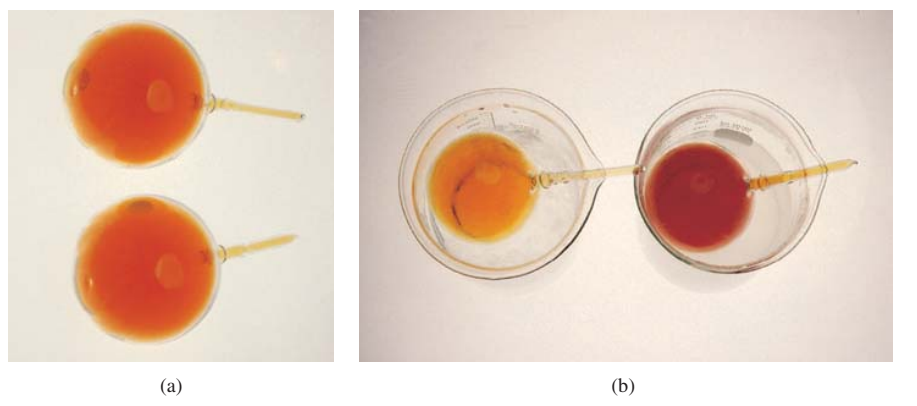
\includegraphics[width=0.5\textwidth,height=2in]{Screenshot 2023-03-22 233354.png}
\end{center}
(a) Two bulbs 
containing a mixture of $\ce{NO2}$ and $\ce{N2O4}$ gases at equilibrium. 
(b) When one bulb is immersed  in ice water (left), its color  becomes lighter, indicating the  formation of colorless $\ce{N2O4}$ gas. 
When the other bulb is immersed  in hot water, its color darkens, 
indicating an increase in $\ce{NO2}$.

$$
\mathrm{N}_2 \mathrm{O}_4(g) \rightleftharpoons 2 \mathrm{NO}_2(g)
$$
The forward reaction is endothermic (absorbs heat, $\Delta H^{\circ}>0$ ):
$$
\text { heat }+\mathrm{N}_2 \mathrm{O}_4(g) \longrightarrow 2 \mathrm{NO}_2(g)$$ 
$$\Delta H^{\circ}=58.0 \mathrm{~kJ} / \mathrm{mol}
$$
so the reverse reaction is exothermic (releases heat, $\Delta H^{\circ}<0$ ):
$$
2 \mathrm{NO}_2(g) \longrightarrow \mathrm{N}_2 \mathrm{O}_4(g)+\text { heat }$$  
$$\Delta H^{\circ}=-58.0 \mathrm{~kJ} / \mathrm{mol}
$$
At equilibrium at a certain temperature, the heat effect is zero because there is no net reaction. If we treat heat as though it were a chemical reagent, then a rise in temperature "adds" heat to the system and a drop in temperature "removes" heat from the system. As with a change in any other parameter (concentration, pressure, or volume), the system shifts to reduce the effect of the change. Therefore, a temperature increase favors the endothermic direction of the reaction (from left to right of the equilibrium equation), which decreases $\left[\mathrm{N}_2 \mathrm{O}_4\right]$ and increases $\left[\mathrm{NO}_2\right]$. A temperature decrease favors the exothermic direction of the reaction (from right to left of the equilibrium equation), which decreases $\left[\mathrm{NO}_2\right]$ and increases $\left[\mathrm{N}_2 \mathrm{O}_4\right]$. Consequently, the equilibrium constant, given by
$$
K_{\mathrm{c}}=\frac{\left[\mathrm{NO}_2\right]^2}{\left[\mathrm{~N}_2 \mathrm{O}_4\right]}
$$
increases when the system is heated and decreases when the system is cooled.


\begin{Box1}{}
    {\large     \textbf{A temperature increase favors an endothermic reaction, and a temperature decrease favors an exothermic reaction.}}
\end{Box1}

\section{The Effect of a Catalyst}
\begin{itemize}
    \item A catalyst enhances the rate of a reaction by lowering the activation energy of the reaction. 
    \item However, a catalyst lowers the activation energy of the forward reaction and the reverse reaction to the same extent.
    \item The presence of a catalyst does not alter the equilibrium constant, nor does it shift the position of an equilibrium system. 
    \item Adding a catalyst to a reaction mixture that is not at equilibrium will simply cause the mixture to reach equilibrium sooner. The same equilibrium mixture could be obtained without the catalyst, but we might have to wait much longer for it to happen.
\end{itemize}


\section{Summary of Factors That May Affect the Equilibrium Position}
\begin{itemize}
    \item Only a change in temperature changes the value of the equilibrium constant. 
    \item Changes in concentration, pressure, and volume can alter the equilibrium concentrations of the reacting mixture, but they cannot change the equilibrium constant as long as the temperature does not change.
    \item A catalyst can speed up the process, but it has no effect on the equilibrium constant or on the equilibrium concentrations of the reacting species.
\end{itemize}

\section{Haber Process}
\begin{center}
    $\ce{N2 (g) + 3H2 (g) <=> 2NH3 (g)}$ $\mathrm{\Delta H^{o} = -92.6 kJ/mol}$
\end{center}
\begin{itemize}
    \item The combination of high-pressure, high-temperature conditions and the proper catalyst is the most efficient way to reduce ammonia on a large scale.
    \item  \textbf{Temparature:} $400-500^o$ C \\
          \textbf{Pressure:} 600 atm \\
          \textbf{Catalyst:}  $\ce{SiO2 + Al2O3 + Fe3O4}$ with $\ce{K2O}$ as a promoter
\end{itemize}


\tikzstyle{box} = [rectangle, text width = 2.1cm,
minimum height = 2cm, text centered, draw=blue]
\tikzstyle{arrow} = [thick, ->, >=stealth]

\begin{figure}[h]
    \centering
    \begin{tikzpicture}[node distance = 2cm]
        \node (comp) [box] {Compressor};
        \node (rxnChamber) [box, right of = comp, xshift=1.5cm] {Reaction Chamber (catalysts)};
        \node (amonia) [box, below of=rxnChamber, yshift=-1cm] {Amonia Condenser};
        \node (storage) [box, below of=amonia, yshift=-1cm] {Storage Tanks};
        \node (foo) [left of=comp, xshift=-1cm] {};
        
        \draw [arrow] (foo) -- node[anchor=south] {$\ce{H2 + N2}$} (comp) coordinate[midway] (aux){};
        \draw [arrow] (comp) -- (rxnChamber);
        \draw [arrow] (rxnChamber) -- node[anchor=east] {$\ce{NH3 + H2 + N2}$} (amonia);
        \draw [arrow] (amonia) -- node[anchor=east] {Liquid $\ce{NH3}$} (storage);
        \draw [arrow] (storage) -| node[anchor=south, xshift=2cm] {Unreacted} node[anchor=north, xshift=2cm] {$\ce{H2 + N2}$} (aux);
    \end{tikzpicture}
\end{figure}
\textbf{Schematic diagram of the Haber process for ammonia synthesis. The heat
generated from the reaction is used to heat the incoming gases.}
\begin{figure}[h]
    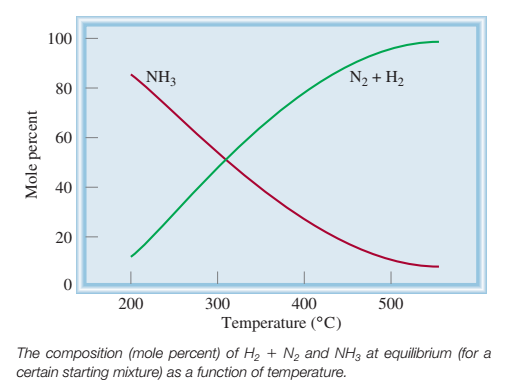
\includegraphics[width=.5\textwidth]{Screenshot 2023-03-23 002349.png}
\end{figure}
\begin{figure}[h]
    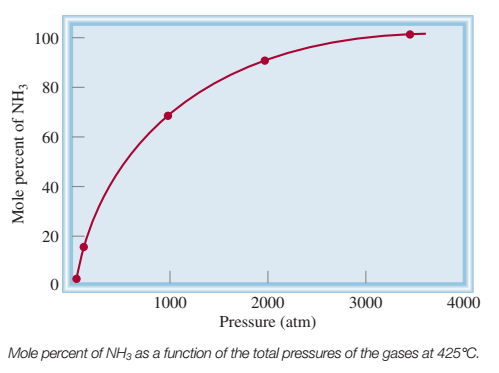
\includegraphics[width=.5\textwidth]{Screenshot 2023-03-23 002340.png}
\end{figure}


\section{Why High Temperature?}
\begin{itemize}
    \item High-temperature operation is costly and the yield of $\ce{NH3}$ is low. The justification for this choice is that the rate of $\ce{NH3}$ production increases with increasing temperature.
    \item Commercially, faster production of $\ce{NH3}$ is preferable even if it means a lower yield and higher operating cost.
\end{itemize}
\end{document}